\section{Implementación}
\rhostart{}

La implementación del programa se realizó mediante el lenguaje de programación C. Las funciones necesarias fueron implementadas en archivos separados según su funcionalidad. El código fue compilado a través de un \texttt{Makefile}, el cual se encuentra en el directorio raíz.

\subsection{Estructura de directorios}
Dentro del directorio \texttt{src} se encuentran los siguientes archivos:

\begin{itemize}
    \item \texttt{errors.c}: Contiene las funciones de gestión de errores.
    \item \texttt{files.c}: Contiene las funciones de gestión de archivos.
    \item \texttt{graph.c}: Contiene las funciones de gestión de grafos.
    \item \texttt{hash.c}: Contiene las funciones de gestión de tablas hash.
    \item \texttt{link\_list.c:} Contiene las funciones de gestión de listas enlazadas.
    \item \texttt{main.c}: Contiene el código principal del programa.
    \item \texttt{page\_rank.c}: Contiene las funciones de calculación de PageRank.
    \item \texttt{reverse\_index.c}: Contiene las funciones de gestión del índice invertido.
    \item \texttt{stop\_words.c}: Contiene las funciones de gestión de stop words.
    \item \texttt{timer.c}: Contiene las funciones de gestión de tiempo de ejecución.
    \item \texttt{utilities.c}: Contiene las funciones de utilidad del programa.
\end{itemize}

Por otro lado, en la carpeta \texttt{testing} se encuentran archivos para el testeo del programa:
\begin{itemize}
    \item \texttt{spanish.txt}: Contiene una lista de stop words en español.
    \item \texttt{test.txt}: Script de \textit{Python} que recupera de \textit{Wikipedia} artículos aleatorios.
\end{itemize}


\subsection{Estructuras de datos}

\subsubsection{Índice invertido}
Para el índice invertido se optó finalmente por utilizar una \textbf{tabla hash} para almacenar las palabras, permitiendo así una búsqueda de orden $O(1)$. Sin embargo, acá surgieron algunos inconvenientes, como la necesidad de manejar posibles colisiones y el límite de memoria que trae consigo los arreglos. Para solucionar esto, se optó que cada celda de esta tabla hash contenga una \textbf{lista enlazada simple}, en la cual será en donde realmente se almacenarán las palabras asociadas a un hash key. Esto permite una búsqueda más eficiente y sin un límite de memoria.

Por otro lado, para poder relacionar un archivo con una palabra se hizo que cada palabra además almacene consigo otra \textbf{lista enlazada simple}, en la cual se almacenarán los archivos que contienen dicha palabra.

\begin{figure}[h!]
    \centering
    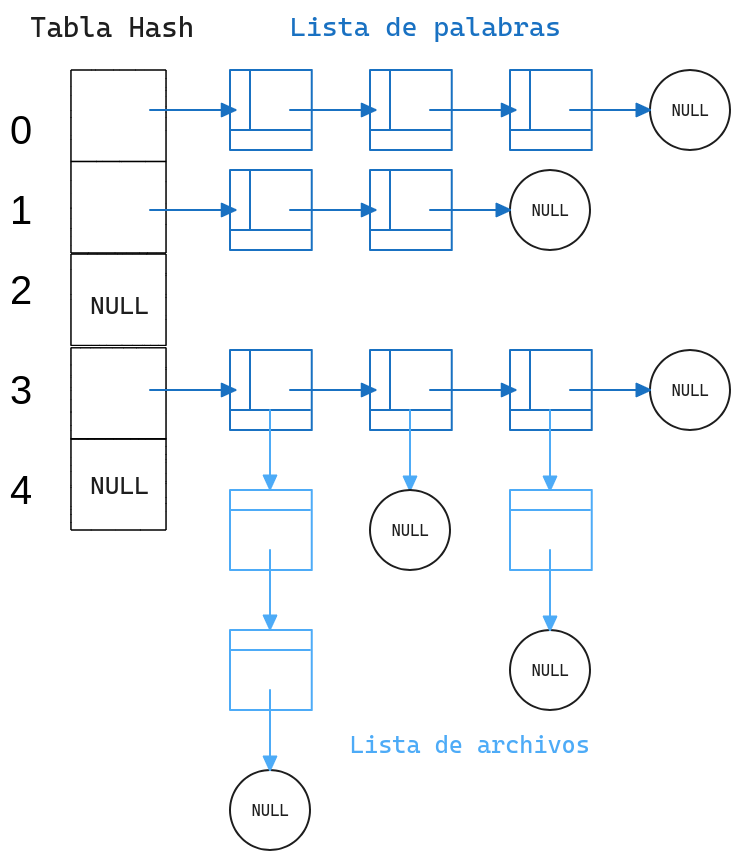
\includegraphics[width=0.3\textwidth]{src/figures/reverse_index.png}
    \caption{Esquema de la estructura de datos del índice invertido}
\end{figure}

\subsubsection{Grafos}

\subsection{PageRank}

\subsection{Manejo de archivos}
Para el manejo de archivos se optó por utilizar una \textbf{lista enlazada simple} para almacenar los archivos, en la cual cada archivo se almacena en una celda de la lista. Esto permite una búsqueda más eficiente y sin un límite de memoria. Además, para poder identificar y procesar los archivos del directorio y sus sub-directorios se utilizó la librería \textbf{dirent.h}.

La librería \textbf{dirent.h} es una librería de C que permite leer los archivos de un directorio, y que proporciona una estructura llamada \textbf{struct dirent} que contiene información sobre cada archivo, como por ejemplo su nombre (con extensión), su tipo (archivo o directorio) y su identificador (ID).

En el caso de existir un sub-directorio dentro del directorio de entrada, se procesará recursivamente, añadiendo cada archivo que se encuentre en dicho directorio a la lista de archivos.

Por último para poder identificar los archivos que contienen texto plano, se utilizó una función para extraer el nombre sin extensión y a su vez verificar si el archivo es de texto plano a traves de su extensión.

\subsection{implementaciones extras}
Se implementó un temporizador para medir los tiempos de ejecución de las funciones y así analizar y mejorar el código(solo para testing).

También se utilizó \textbf{mergeSort} para ordenar (de mayor a menor) el PageRank de los archivos, para tener una mejor visualización de los resultados.